\chapter{USB 2.0}
  %INTRODUCCION

  \section{Introducción}
  El Bus Serie Universal, o USB, (acrónimo del inglés {\it Universal Serial Bus})
  es uno de los ejes centrales del presente trabajo. Por este motivo, se hace a
  continuación una revisión de los aspectos más relevantes de la norma.\\

  Las norma USB está fundada en la revisión 2.0 de las
  \href{www.usb.org}{\it Especificaciones USB}, publicadas en Abril del año
  2000.\\

  Para describir un sistema USB, se abordan tres temáticas diferentes, pero
  relacionadas una con la otra:

  \begin{itemize}
    \item Interconexión USB
    \item \host
    \item Dispositivos USB
  \end{itemize}

  El objetivo principal de un sistema USB puede resumirse como la correcta
  comunicación entre el \host ~y los distintos dispositivos USB, a traveś de
  la interconexión USB. El objetivo particular de la revisión 2.0 de la norma es
  la de brindar un mayor ancho de banda, incorporando a las velocidades baja
  ({\it low speed}) y completa ({\it full speed}) una opcion de alta velocidad
  ({\it high speed}). Esto supone agregar a las comunicación de 1.5 Mbps y 12
  Mbps, una variante que alcanza los 480 Mbps.\\

  Se describen, entonces, a continuación.

  \section{Host USB}
  Todo sistema de comunicación USB posee un compoennete único, escencial,
  fundamental. Este componente es el \host.\\

  La palabra {\it Host} viene de la voz inglesa y su traducción tiene muchas
  acepciones. La traducción más común es la de anfitrión. Sin embargo, también
  se puede nombrar así a un presentador de televisión o a un portador.\\

  Si se habla de redes, un {\it host} es cada uno de los dispositivos que se
  conectan a ella y de los cuales un servidor puede tomar o brindar información
  o recursos.\\

  No obstante, en un sistema USB, ninguna de estas acepciones permite describir
  del todo lo que significa un \host. Es por eso que quién escribe se ha tomado
  la libertad de usar la palabra inglesa.\\

  El \host debe ser capaz de reconocer cuando un dispositivo es conectado,
  colectar la descripción del mismo, negociar con él la forma de comunicarse,
  enumerarlo, administrar el flujo de la información, emitir las turnos de uso
  del bus, reconocer el estado y llevar la estadística de la actividad del
  bus.\\

  Todo esto, se lleva a cabo a través del Controlador del Host, que puede estar
  compuesto por hardware, firmware y/o software, pero que se aloja en el
  \host.\\

  \section{Dispositivos USB}
  Existen dos tipos fundamentales de {\it Dispositivos USB}, tal como los define
  la norma USB, a saber, los \hubs (textualmente, {\it USB Hubs}) y
  las funciones. También existen dispositivos compuestos, en los que se integran
  tanto un \hub como funciones.\\

  \subsection{\Hub}
  Un \hub es un dispositivo en el que confluyen multiples conexiones, brindando
  la posibilidad al usuario de agregar diversos dispositivos al mismo sistema.
  Los puntos de conexión se denominan puertos. En otras palabras, un hub es
  un multiplicador de puertos, convirtiendo un solo puerto de subida en varios
  puertos de bajada.\\

  Especificamente, un \hub 2.0 consiste de tres componentes: un controlador, un
  repetidor y un traductor de transacciones. El repetidor es un switch que
  conecta los múltiples puertos de bajada con el de subida. Suele poseer
  hardware adicional que brinda la posibilidad de emitir señales de reset y de
  suspender/continuar. El traductor de transacciones se encarga de las
  comunicaciones con dispositivos rio abajo a baja o media velocidad, y a alta
  velocidad con el \host, rio arriba. El controlador brinda la capacidad de
  comunicación con el \host y, a traves de comandos de estado y control
  específicos, le permite a \host configurar cada \hub.\\

  \subsection{Funciones}
  Se denomina función a todo aquel dispositivo que puede recibir o emitir
  información a través del bus. Por lo general, suelen ser periféricos que se
  conectan con un cable a un \hub, pero también existen dispositivos combinados
  que no solo tienen alguna función, sino que además incorpora un \hub y brinda
  puertos adicionales para otras funciones.\\

  Cada función posee información que describe sus capacidades y los
  requerimientos de sistema que necesita para operar. Antes de comenzar a
  comunicar, el \host realizar la configuración, que consiste en la selección
  del ancho de banda con la que el dispositivos debe operar, la dirección del
  puerto del dispositivo y seleccionar las opciones específicas de cada
  función.\\

  Una función, a su vez está compuesta de \eps, que es la porción logica mínima
  que maneja un sistema USB. Un \ep solo puede tener un dirección, es decir, un
  conjunto númerico único que lo identifica con respecto a cualquier otro
  dispositivo conectado al bus, y sentido, o sea, de entrada hacia el \host o de
  salida desde este último.\\

  \section{Interconexion USB}
  Cuando se habla de interconexión, se hace referencia a la forma en la que los
  distintos componentes se conectan y cómo se comunican entre ellos. Para ello,
  se detalla a continuación la topología USB, es decir, el modelo de conexión
  entre el host y los dispositivos; el flujo de datos, o sea, la manera en la
  que los datos viajan a través del sistema entre las fuentes de información y
  los consumidores de ella; la lista de trabajo de cada dispositivo y la
  relación entre las diferentes capas de cada dispositivo.\\

  Se procede a explicar con más detalle algunas de estas cuestiones.\\

    \subsection{Topología USB}
    El USB es un sistema centrado en el \host. Él es el maestro, el que da las
    órdenes o los turnos para que cada dispositivos pueda transmitir o recibir
    información. Cada dispositivo responderá consiguientemente al pedido por
    por parte del \host.\\

    La topología es, entonces, en estrella por niveles, donde el \host es el
    centro y cada dispositivo es una extensión. Los niveles se separa a través
    de distribuidores, que sirven para ampliar la red y son los centro de cada
    nuevo nivel.\\

    \begin{figure}
      \centering
      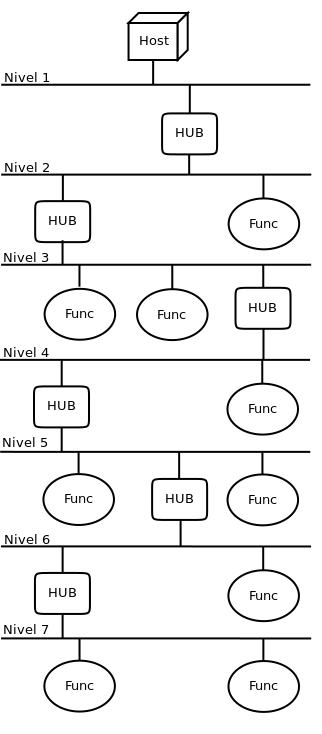
\includegraphics[width=0.25\textwidth ]{topologia.png}
      \caption{Topología USB}
      \label{}
    \end{figure}

    Debido a las restricciones de tiempo y ancho de banda impuestas por las
    especificaciones de la norma USB 2.0, no puede existir más que 7 niveles
    en un sistema USB, incluido el nivel del \host, por lo que no puede existir
    un distribuidor en el último nivel.\\

    \subsection{Protocolo}


    \subsection{Flujo de datos}
      \subsubsection{Dirección de datos}
      El sistema USB, como se describe anteriormente, posee un modelo centrado
      en el \host, y este debe ser único. Él es el dspositivo central, que
      recibe y/o emite información a cada dispositivo Función o \Hub. Es por
      esto, que toda comunicación se referencia siempre al \host. Es decir, si
      hablamos de una transferencia de entrada, quiere decir que el periférico
      o el dispositivo en cuestión esta enviando datos y estos entran al \host.
      En cambio, una transferencia de salida, es una operación que sale del
      \host y se dirige hacia el dispositivo que la necesita.

      \subsubsection{Tipos de Transferencia}
      Las trasnferencias, ya sean de entrada o de salida, pueden ser de cuatro
      tipos diferentes:

      \begin{itemize}
         \item Transferencias de control:
         \item Transferencias por bultos:
         \item Trasnferencias por interrupción:
         \item Trasnferencias isocrónicas:
      \end{itemize}


  % Desde su primera especificación, lanzada en 1996, hasta la fecha la norma USB
  % ha ido adquiriendo importancia y relevancia, debido a la aceptación que tuvo
  % por parte de los fabricantes y los usuarios.
  %
  % USB, acrónimo de Universal Serial Bus (o Bus Serie Universal, en español) es
  % una norma de comunicación pensada originalmente para comunicar periféricos con
  % la computadora. Sin embargo, hoy en día brinda la posibilidad no solo de
  % obtener diferentes dispositivos que se comunican de manera simple, robusta y
  % veloz con cualquier PC, sino que, además permite al usuario obtener una fuente
  % segura y confiable de energía para cualquier aparato electrónico que así lo
  % requiera. Por este motivo, se está transformado en la única de comunicación de
  % cualquier dispositivo de consumo masivo.
  %
  % Observando las especificaciones, USB es una comunicación que posee una
  % complejidad mucho mayor que la que presentan los sistemas serie o paralelo
  % tradicionales. Introduce nuevos términos, tales como extremos,
  % isocronismo o enumeración, y le da nuevo significado a palabras ya conocidas,
  % como configuración, interrupción o interfaz. No obstante esto, está muy bien
  % separada por capas que facilitan el trabajo de la implementación del sistema
  % y pueden ser vistas como sistemas aislados.
  %
  % A continuación se describen algunos detalles técnicos de esta norma, que son
  % parte fundamental del trabajo realizado.
  %
  % \section{La especificación USB 2.0}
  % En el año 2000, el comité conformado por seis de las más grandes compañías de
  % la industria informática del momento, Compaq, Intel, Microsoft, NEC, Lucent,
  % Hewlett-Packard y Philips; lanzó el documento final que describe las
  % especificaciones de la versión USB 2.0. El documento puede ser descargado de
  % forma gratuita desde el sitio: \href{http://www.usb.org}{www.usb.org}.
  %
  % \section{Conceptos Fundamentales}
  % La norma USB 2.0 incorpora y modifica términos y conceptos que es conveniente
  % conocer antes de una descripción más profunda de los elementos de interés para
  % el presente trabajo.
  %   \subsection{Dispositivos que intrevienen}
  %     \subsubsection{\host}
  %     Es el dispositivo central de la comunicación USB. Solo puede existir solo
  %     un \host y es la PC, o el dispositivo que contenga el \host~\controller.
  %     Es quien asigna las direcciones de cada dispositivo y solicita alguna
  %     acción a los \devices.
  %
  %     \subsubsection{\device}
  %     Es toda unidad lógica o física que realiza una función.
  %
  %     \subsubsection{\hub}
  %     Es un \device que permite conectar una o varias funciones, aguas abajo.
  %
  %     \subsubsection{\function}
  %     Cualquier \device que agregues capacidades al \host.
  %
  %     \subsubsection{\ep}
  %     Es la porción direccional de \device que sea emisor o destino de
  %     información respecto al \host.
  %
  %     \subsubsection{\controller}Se refiere a la interfaz USB, compuesta del
  %     software y hardware que posibilitan la comunicación.
  %
  % \section{Topología USB}
  % Cualquier sistema de comunicación USB posee una topología en estrella por
  % niveles. Cada centro de los niveles de la estrella es un \hub.
  % En el nivel superiorse encuentra el \host%BUSCAR SINONIMO
  % , el \hub raíz, y luego, por cada \hub adicional, se agrega un nuevo nivel.
  % Debido a las restricciones temporales, no puede haber más de 7 niveles.
  % Cada \device no puede enviar o recibir información sin la solicitud expresa
  % del \host.
  %
  % % \section{Reseña histórica}
  % %
  % % El 11 de Noviembre de 1994, un comité de trabajo compuesto por ingenieros y
  % % desarrolladores de siete de las grandes compañías de la industría electrónica
  % % e informática del momento: Compaq, Hewlett-Packard, Intel, Lucent, Microsoft,
  % % NEC y Philips; lanzó los lineamientos fundamentales de trabajo sobre un nuevo
  % % estándar de interconexión entre computadoras personales y dispositivos
  % % periféricos. El objetivo principal fué definir las especificaciones que se
  % % tendrían en cuenta a fin de realizar una correcta comunicación entre una PC y
  % % el teléfono, que sea facil de usar y que brinde una expansión de los puertos
  % % que permita a los nuevos dispositivos periféricos que iban naciendo ser
  % % conectados sin la necesidad de agrandar en forma infinita el hardware
  % % necesario.\\
  % %
  % % Finalmente, el 15 de Enero de 1996 se publico la version 1.0 de la norma USB.
  % % En su primera versión contemplaba dos modos de operación, low-speed de
  % % \SI{1.5}{\mega\byte/\second} y full-speed, que opera a
  % % \SI{12}{\mega\byte/\second}.\\
  % %
  % % Sin embargo, la gran evolución en el desempeño de las computadoras que se
  % % comercializaban a gran escala, junto con el advenimiento de periféricos cada
  % % vez más sofisticados que posibilitaban aplicaciones de mayor ancho de banda,
  % % como por ejemplo la imagen digital, puso la necesidad de incorporar una mayor
  % % velocidad y eficiencia a la norma USB. De esta forma, el 27 de Abril del 2000,
  % % se lanzó la versión USB 2.0, que agregaba un modo más de comunicación,
  % % high-speed, que posibilita el envío y recepción de hasta
  % % \SI{480}{\mega\byte/\second}
  % %
  % % \section{Descripción del sistema}
  % %
  % %   Un sistema USB está compuesta por varios conceptos importantes, como ser la
  % %   conexión fisica, potencia, protocolo, robustez de la comunicación, etc. Sin
  % %   embargo, debido al interés del presente trabajo, se detallarás solo algunos
  % %   aspectos importantes con respecto a las componentes de un sistema USB, su
  % %   topología, el flujo de datos y algunos aspectos de la red, descripta
  % %   mediante el modelo OSI
